%%%%%%%%%%%%%%%%%%%%%%%%%%%%%%%%%%%%%%%%%%%%%%%%%%%%%%%%%%%%%
%%
%%
%%     NPR's  Nature template...  
%%     v1.0.0   Thu Dec  8 19:05:57 EST 2016
%%                                                                         
%%
%%%%%%%%%%%%%%%%%%%%%%%%%%%%%%%%%%%%%%%%%%%%%%%%%%%%%%%%%%%%%
\documentclass{nature}
%\documentclass{natureprintstyle}

\usepackage{graphicx,psfig,fancyhdr,natbib,subfigure}
\usepackage{epsfig, psfig, epsf}
\usepackage{amsmath, cancel}
\usepackage{amssymb}
%\usepackage{lscape}
\usepackage{dcolumn}% Align table columns on decimal point
\usepackage{bm}% bold math
\usepackage{hyperref,ifthen}
\usepackage{verbatim}



%%%%%%%%%%%%%%%%%%%%%%%%%%%%%%%%%%%%%%%%%%%
%       define Journal abbreviations      %
%%%%%%%%%%%%%%%%%%%%%%%%%%%%%%%%%%%%%%%%%%%
\def\nat{Nat} \def\apjl{ApJ~Lett.} \def\apj{ApJ}
\def\apjs{ApJS} \def\aj{AJ} \def\mnras{MNRAS}
\def\prd{Phys.~Rev.~D} \def\prl{Phys.~Rev.~Lett.}
\def\plb{Phys.~Lett.~B} \def\jhep{JHEP}
\def\npbps{NUC.~Phys.~B~Proc.~Suppl.} \def\prep{Phys.~Rep.}
\def\pasp{PASP} \def\aap{Astron.~\&~Astrophys.} \def\araa{ARA\&A}
\def\jcap{\ref@jnl{J. Cosmology Astropart. Phys.}} 
\def\nar{New~A.R.} 

\newcommand{\preep}[1]{{\tt #1} }

%%%%%%%%%%%%%%%%%%%%%%%%%%%%%%%%%%%%%%%%%%%%%%%%%%%%%
%              define symbols                       %
%%%%%%%%%%%%%%%%%%%%%%%%%%%%%%%%%%%%%%%%%%%%%%%%%%%%%
\def \Mpc {~{\rm Mpc} }
\def \Om {\Omega_0}
\def \Omb {\Omega_{\rm b}}
\def \Omcdm {\Omega_{\rm CDM}}
\def \Omlam {\Omega_{\Lambda}}
\def \Omm {\Omega_{\rm m}}
\def \ho {H_0}
\def \qo {q_0}
\def \lo {\lambda_0}
\def \kms {{\rm ~km~s}^{-1}}
\def \kmsmpc {{\rm ~km~s}^{-1}~{\rm Mpc}^{-1}}
\def \hmpc{~\;h^{-1}~{\rm Mpc}} 
\def \hkpc{\;h^{-1}{\rm kpc}} 
\def \hmpcb{h^{-1}{\rm Mpc}}
\def \dif {{\rm d}}
\def \mlim {m_{\rm l}}
\def \bj {b_{\rm J}}
\def \mb {M_{\rm b_{\rm J}}}
\def \mg {M_{\rm g}}
\def \mi {M_{\rm i}}
\def \qso {_{\rm QSO}}
\def \lrg {_{\rm LRG}}
\def \gal {_{\rm gal}}
\def \xibar {\bar{\xi}}
\def \xis{\xi(s)}
\def \xisp{\xi(\sigma, \pi)}
\def \Xisig{\Xi(\sigma)}
\def \xir{\xi(r)}
\def \max {_{\rm max}}
\def \gsim { \lower .75ex \hbox{$\sim$} \llap{\raise .27ex \hbox{$>$}} }
\def \lsim { \lower .75ex \hbox{$\sim$} \llap{\raise .27ex \hbox{$<$}} }
\def \deg {^{\circ}}
%\def \sqdeg {\rm deg^{-2}}
\def \deltac {\delta_{\rm c}}
\def \mmin {M_{\rm min}}
\def \mbh  {M_{\rm BH}}
\def \mdh  {M_{\rm DH}}
\def \msun {M_{\odot}}
\def \z {_{\rm z}}
\def \edd {_{\rm Edd}}
\def \lin {_{\rm lin}}
\def \nonlin {_{\rm non-lin}}
\def \wrms {\langle w_{\rm z}^2\rangle^{1/2}}
\def \dc {\delta_{\rm c}}
\def \wp {w_{p}(\sigma)}
\def \PwrSp {\mathcal{P}(k)}
\def \DelSq {$\Delta^{2}(k)$}
\def \WMAP {{\it WMAP \,}}
\def \cobe {{\it COBE }}
\def \COBE {{\it COBE \;}}
\def \HST  {{\it HST \,\,}}
\def \Spitzer  {{\it Spitzer \,}}
\def \ATLAS {VST-AA$\Omega$ {\it ATLAS} }
\def \BEST   {{\tt best} }
\def \TARGET {{\tt target} }
\def \TQSO   {{\tt TARGET\_QSO}}
\def \HIZ    {{\tt TARGET\_HIZ}}
\def \FIRST  {{\tt TARGET\_FIRST}}
\def \zc {z_{\rm c}}
\def \zcz {z_{\rm c,0}}


\newcommand{\sqdeg}{deg$^{-2}$}
\newcommand{\lya}{Ly$\alpha$\ }
%\newcommand{\lya}{Ly\,$\alpha$\ }
\newcommand{\lyaf}{Ly\,$\alpha$\ forest}
%\newcommand{\eg}{e.g.~}
%\newcommand{\etal}{et~al.~}
\newcommand{\cii}{C\,{\sc ii}\ }
\newcommand{\ciii}{C\,{\sc iii}]\ }
\newcommand{\civ}{C\,{\sc iv}\ }
\newcommand{\SiIV}{Si\,{\sc iv}\ }
\newcommand{\mgii}{Mg\,{\sc ii}\ }
\newcommand{\feii}{Fe\,{\sc ii}\ }
\newcommand{\feiii}{Fe\,{\sc iii}\ }
\newcommand{\caii}{Ca\,{\sc ii}\ }
\newcommand{\halpha}{H\,$\alpha$\ }
\newcommand{\hbeta}{H\,$\beta$\ }
\newcommand{\oi}{[O\,{\sc i}]\ }
\newcommand{\oii}{[O\,{\sc ii}]\ }
\newcommand{\oiii}{[O\,{\sc iii}]\ }
\newcommand{\heii}{[He\,{\sc ii}]\ }
\newcommand{\nii}{N\,{\sc ii}\ }
\newcommand{\nv}{N\,{\sc v}\ }

%% From:: /cos_pc19a_npr/LaTeX/proposals/JWST/JWST_ERS/Proposal/lines.tex
%%  
\newcommand{\imw}{$i$--$W3$}
\newcommand{\imwf}{$i$--$W4$}
\newcommand{\rmwf}{$r$--$W4$}
\newcommand{\imwt}{$i$--$W2$}
\newcommand{\wtmwf}{$W3$--$W4$}
%\newcommand{\kms}{km s$^{-1}$}
\newcommand{\cmN}{cm$^{-2}$}
\newcommand{\cmn}{cm$^{-3}$}
%\newcommand{\msun}{M$_{\odot}$}
\newcommand{\lsun}{L$_{\odot}$}
\newcommand{\lam}{$\lambda$}
\newcommand{\mum}{$\mu$m}
\newcommand{\ebv}{$E(B$$-$$V)$}
%\newcommand{\heii}{\mbox{He\,{\sc ii}}}
\newcommand{\cv}{\mbox{C\,{\sc v}}}
%\newcommand{\civ}{\mbox{C\,{\sc iv}}}
%\newcommand{\ciii}{\mbox{C\,{\sc iii}}}
%\newcommand{\cii}{\mbox{C\,{\sc ii}}}
%\newcommand{\nv}{\mbox{N\,{\sc v}}}
\newcommand{\niv}{\mbox{N\,{\sc iv}}}
\newcommand{\niii}{\mbox{N\,{\sc iii}}}
%\newcommand{\oi}{\mbox{O\,{\sc i}}}
%\newcommand{\oii}{\mbox{O\,{\sc ii}}}
%\newcommand{\oiii}{\mbox{[O\,{\sc iii}]}}
\newcommand{\oiv}{\mbox{O\,{\sc iv}}}
\newcommand{\ov}{\mbox{O\,{\sc v}}}
\newcommand{\ovi}{\mbox{O\,{\sc vi}}}
\newcommand{\ovii}{\mbox{O\,{\sc vii}}}

%\newcommand{\feii}{\mbox{Fe\,{\sc ii}}}
%\newcommand{\feiii}{\mbox{Fe\,{\sc iii}}}
%\newcommand{\mgii}{\mbox{Mg\,{\sc ii}}}
\newcommand{\neii}{[Ne\,{\sc ii}]\ }
\newcommand{\neiii}{[Ne\,{\sc ii}]\ }
\newcommand{\nev}{Ne\,{\sc v}\ }
\newcommand{\nevi}{[Ne\,{\sc vi}]\ }
\newcommand{\neviii}{\mbox{Ne\,{\sc viii}}}
\newcommand{\aliii}{\mbox{Al\,{\sc iii}}}
\newcommand{\siii}{\mbox{Si\,{\sc ii}}}
\newcommand{\siiii}{\mbox{Si\,{\sc iii}}}
\newcommand{\siiv}{\mbox{Si\,{\sc iv}}}
%\newcommand{\lya}{\mbox{Ly$\alpha$}}
%\newcommand{\lyb}{\mbox{Ly$\beta$}}
\newcommand{\hi}{\mbox{H\,{\sc i}}}
\newcommand{\snine}{\mbox{[S\,{\sc ix}]}}
\newcommand{\sivi}{\mbox{[Si\,{\sc vi}]}}
\newcommand{\sivii}{\mbox[{Si\,{\sc vii}]}}
\newcommand{\siix}{\mbox{[Si\,{\sc ix}]}}
\newcommand{\six}{\mbox{[Si\,{\sc x}]}}
\newcommand{\sixi}{\mbox{[Si\,{\sc xi}]}}
\newcommand{\caviii}{\mbox{[Ca\,{\sc viii}]}}
\newcommand{\arii}{\mbox{[Ar\,{\sc ii}]}}

%%[Ar II] 6.97
%% [S IX] 1.252 μm 328 
% [Si X] 1.430 μm 351 
% [Si XI] 1.932 μm 401 
% [Si VI] 1.962 μm 167 
% [Ca VIII] 2.321 μm 128 
% [Si VII] 2.483 μm 205 
% [Si IX] 3.935 μm 303
% [Ar II] 6.97


%\snine\ at 1.252$\mu$m, \six\ at 1.430$\mu$m, \sixi\ at 1.932$\mu$m, \sivi\ at
%1.962$\mu$m, \caviii\ at 2.321$\mu$m, \sivi\ at 2.483$\mu$m \siix\ at
%3.935$\mu$m and \arii\ at 6.97$\mu$m. 
%%
%% such as [Ne ii]12.8 μm, [Ne v]14.3 μm, [Ne iii]15.5 μm, [S iii]18.7 μm and 33.48 μm, [O iv]25.89 μm and [Si ii]34.8 μm (e.g
%%
%% MIR emission lines like [NeII] and [NeV] are ..
%%
%% Also,  arXiv:astro-ph/0003457v1 
%% [NeV] 14.32um & 24.32um and [NeVI] 7.65um imply an A(V)>160 towards the NLR...
%% [NeIII]15.56um/[NeII]12.81um
%%
%% [Ne V] 14.3, 24.2 μm 97.
%% [Ne II] 12.8 μm
%% [OIV] 26μm
%%



\bibliographystyle{naturemag}


%\title{A Quasar caught in the act of turning off}
\title{A new interpretation of optical and infrared variability in Quasars}

\author{Nicholas~P.~Ross$^{1}$ et al.}  
% Saavik~K.~Ford,$^{7}$, Barry~L.~McKernan$^{7}$,
% Daniel~Stern$^{3}$, Aaron~Meisner$^{2}$, 
% Matthew~Graham$^{4}$, 
% Arjun~Dey$^{5}$ \& David~J.~Schlegel$^{2}$ 
% Andrew~Drake$^{4}$, 
% Roberto~J.~Assef$^{6},
% Mislav~Balokovic$^{6}, 
% Murray~Brightman$^{4}, 
% for the DECaLS Consortium. 


\begin{document}

\maketitle

\begin{affiliations}
  \item Institute for Astronomy, University of Edinburgh, Royal Observatory, Blackford Hill, Edinburgh EH9 3HJ, United Kingdom 
 % \item Department of Astrophysics is located in the Rose Center for Earth and Space, American Museum of Natural History, Central Park West at 79th Street, New York, NY 10024, U.S.A
  %\item Jet Propulsion Laboratory, California Institute of Technology, 4800 Oak Grove Drive, Mail Stop 169-221, Pasadena, CA 91109, USA 
  %\item California Institute of Technology, 1200 East California Boulevard, Pasadena, CA 91125, USA
  %\item Steward Observatory, 933 North Cherry Avenue, Tucson, AZ 85721, U.S.A.
%  \item Universidad Diego Portales, Av Republica 180, Santiago, Regi ́on Metropolitana, Chile}
%  \item Lawrence Berkeley National Laboratory, 1 Cyclotron Road, Berkeley, CA 92420, U.S.A. 
\end{affiliations}


\begin{abstract}
Changing-look quasars are a class of recently identified objects in
which the strong UV continuum and broad optical hydrogen emission
lines associated with unobscured quasars either appear or disappear on
timescales of months to years \cite{LaMassa2015, Runnoe2016, MacLeod2016,
Ruan16}. The physical processes responsible for this behaviour are
still debated, but changes in the black hole accretion rate or
accretion disk structure appear more likely than changes in
obscuration \cite{Hutsemekers2017, Sheng2017}. Here we report on three
epochs of spectroscopy of SDSS J110057.70-005304.5, a quasar at a
redshift of $z=0.378$, whose UV continuum and broad hydrogen emission
lines have dramatically faded over the past $\approx$20 years. The
change in this quasar was initially seen in the infrared, and an
archival spectrum from 2010 shows an intermediate phase of the
transition during which the flux below rest-frame 340nm has
collapsed. This is unique compared to previously published examples of
changing-look quasars, and is best explained by dramatic changes in
the innermost regions of the accretion disk. The optical continuum has
been rising again since mid-2016, leading to a prediction of a rise in
hydrogen emission line flux in the next few months. If our model is
confirmed, the physics of `changing look' quasars are governed by
processes at the innermost stable circular orbit (ISCO) around the
black hole, and the structure of the innermost disk. The easily
identifiably and monitored Changing Look Quasars would then provide a
new probe of the strong gravity regime.
\end{abstract}



%%%%%%%%%%%%%%%%%%%%%%%%%%%%%%%%%%%%%%%%%%%%%%%%%%%%%%%%%%%%%
%%%%%%%%%%%%%%%%%%%%%%%%%%%%%%%%%%%%%%%%%%%%%%%%%%%%%%%%%%%%%
%%
%%   SECTION 1  SECTION 1  SECTION 1  SECTION 1  SECTION 1  SECTION 1  
%%   SECTION 1  SECTION 1  SECTION 1  SECTION 1  SECTION 1  SECTION 1  
%%   SECTION 1  SECTION 1  SECTION 1  SECTION 1  SECTION 1  SECTION 1  
%%
%%%%%%%%%%%%%%%%%%%%%%%%%%%%%%%%%%%%%%%%%%%%%%%%%%%%%%%%%%%%%
%%%%%%%%%%%%%%%%%%%%%%%%%%%%%%%%%%%%%%%%%%%%%%%%%%%%%%%%%%%%%
%\section{Introduction}

The ``Changing-Look'' quasar phenomenon, where the dramatic
disappearance, or appearance, of prominent broad optical emission
lines is seen on month-to-year timescales, is now widely observed,
\cite{LaMassa2015, MacLeod2016, Runnoe2016, Ruan2016, Gezari2017, Rumbaugh2017} 
yet poorly understood. Changes in obscuration are generally
disfavoured \cite{Hutsemekers2017, Sheng2017}, and it is clear that the
CLQs are a key laboratory into understanding accretion physics and the
nature of the AGN broad line region (BLR).
%%
For the AGN accretion disk, the famous $\alpha-$disk model \cite{SS73}
for a optically thick, geometrically thin disk ($h / R \ll 1$, where
$h$ is the vertical scale height of the disk) is known to have serious
short-comings e.g. \cite{Antonucci1999, Koratkar_Blaes1999,
Lawrence2012}. For example, AGN seem to be cooler than they ought to be
\cite[e.g., ][]{Lawrence2012} with the SEDs of AGN showing a universal
near-UV shape, reaching a maximum in $\nu S_{\nu}$ around 1100\AA. 
Such a peak suggests a characteristic temperature of T$\sim$30 000K,
wheres for a thermal model, the characteristic temperature should be
roughly T$\sim$100 000K.  Moreover, constraints from microlensing
observations for the size of the optical emission region \cite[e.g.,
][]{Pooley2007, Morgan2010, Morgan2012, Mosquera2011} suggestion this region is
larger than the one predicted by the standard Shakura-Sunyaev disk.

CLQs have traditionally been discovered by looking for large, $|
\Delta m | >1$ magnitude changes in the optical light curves (e.g. in
the $g$-band). However, we have taken advantage of the ongoing
Near-Earth Object WISE Reactivation mission \cite[NEOWISE-R;
][]{Mainzer2014, Meisner2017, Meisner2017b}, as well as the Dark Energy
Camera Legacy Survey (DECaLS\footnote{{\tt
legacysurvey.org/decamls/}}) in order to discover new CLQs. Our team
is the first to extend this selection to the infrared using NEOWISE-R
mission data. Indeed, we have found a sample of SDSS quasars that show
dramatic decreases in their IR flux over the course of a few
years. These changes are on timescales too short to be considered due
to changes in obscuration, so a new explanation is needed.

In this article we present the $z=0.378$ quasar SDSS
J110057.70-005304.5 (hereafter J110057) that we have observed
transitioning from a blue continuum sloped object to become a regular
galaxy. We present a model that invokes changes at the innermost
stable circular orbit (ISCO) to be the triggering event for the change
in the accretion disk, which along along with the changes in the BELs,
explains a major change to the disk interior to 150$R_{g}$ as well as
the IR light curves. Critically, our model makes predictions to the
future behvaiour of J110057.
 
\begin{figure*}
  \centering
  %% trim=l b r t 
  % 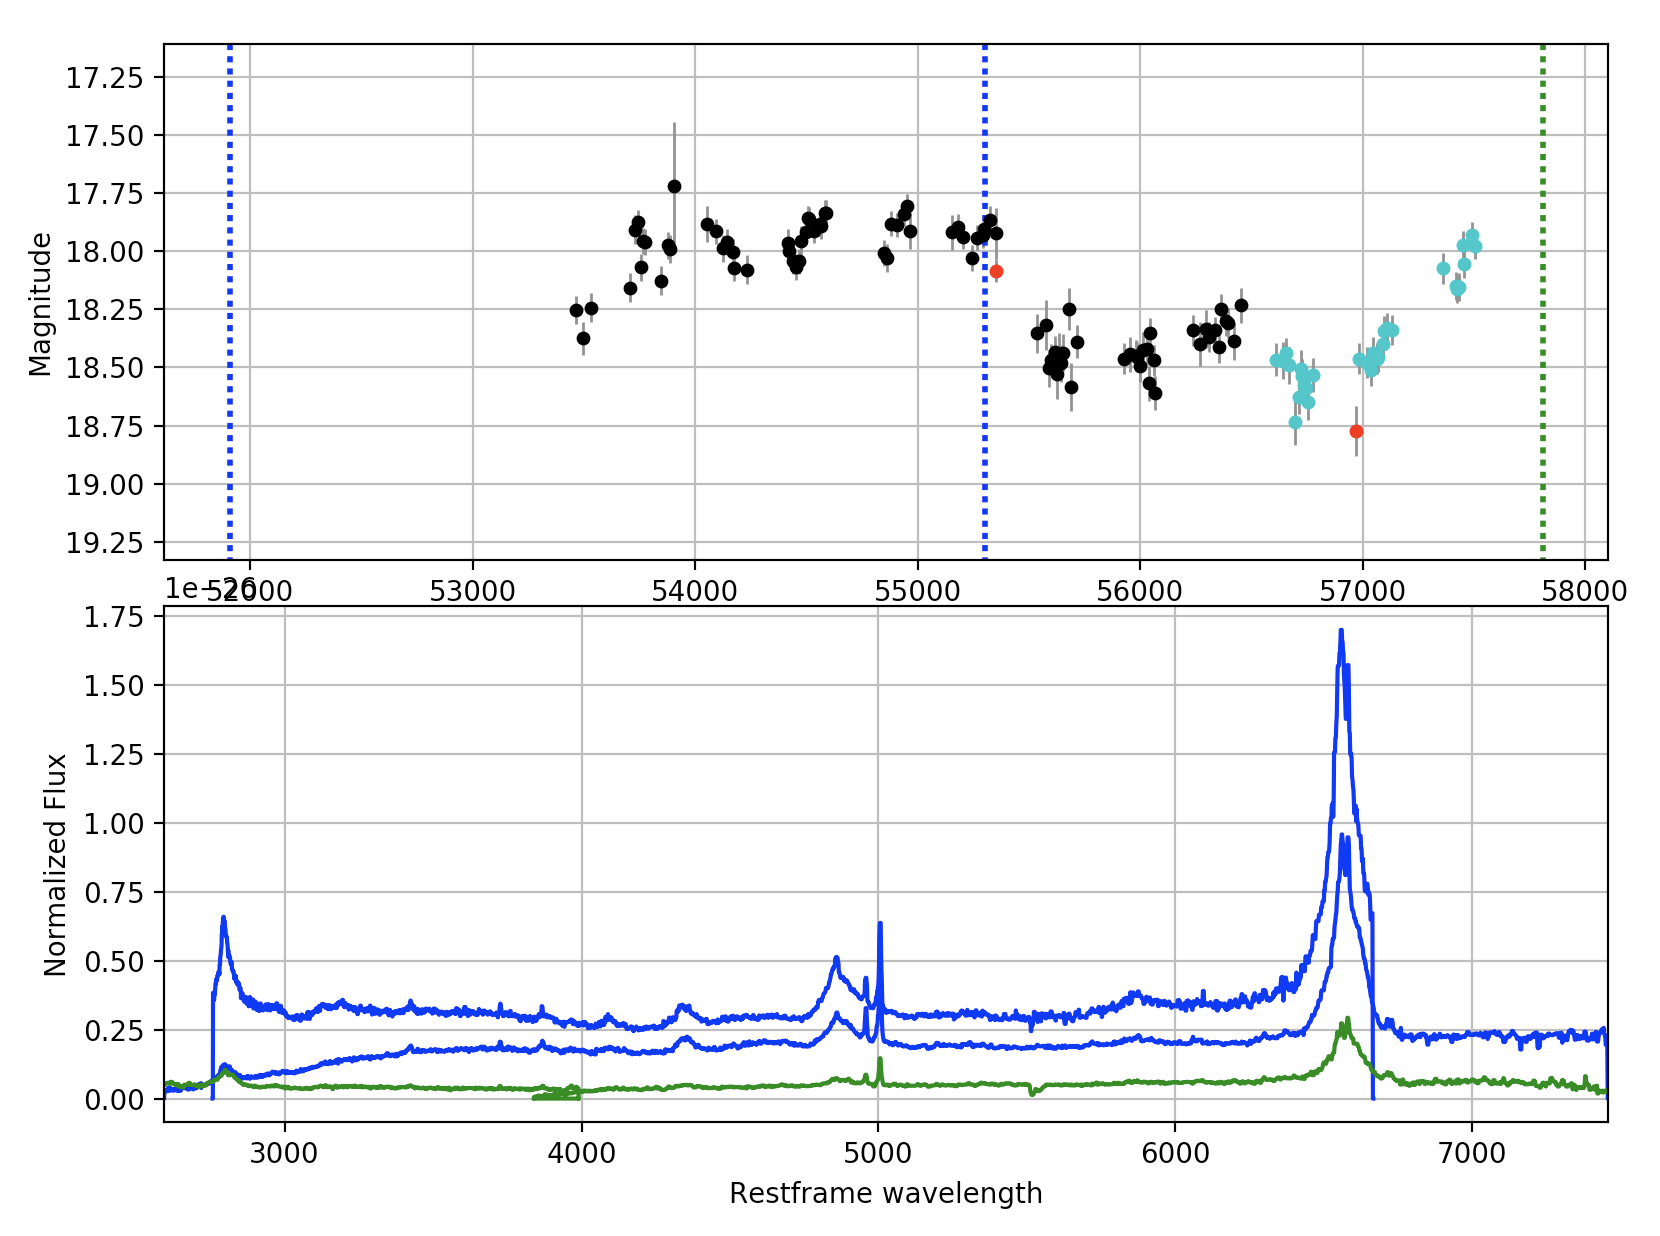
\includegraphics[width=8.00cm, height=7.50cm, trim=0.0cm 0.0cm 0.0cm 0.0cm, clip] {J110057_CRTS_lightcurve_v0pnt1.png}
  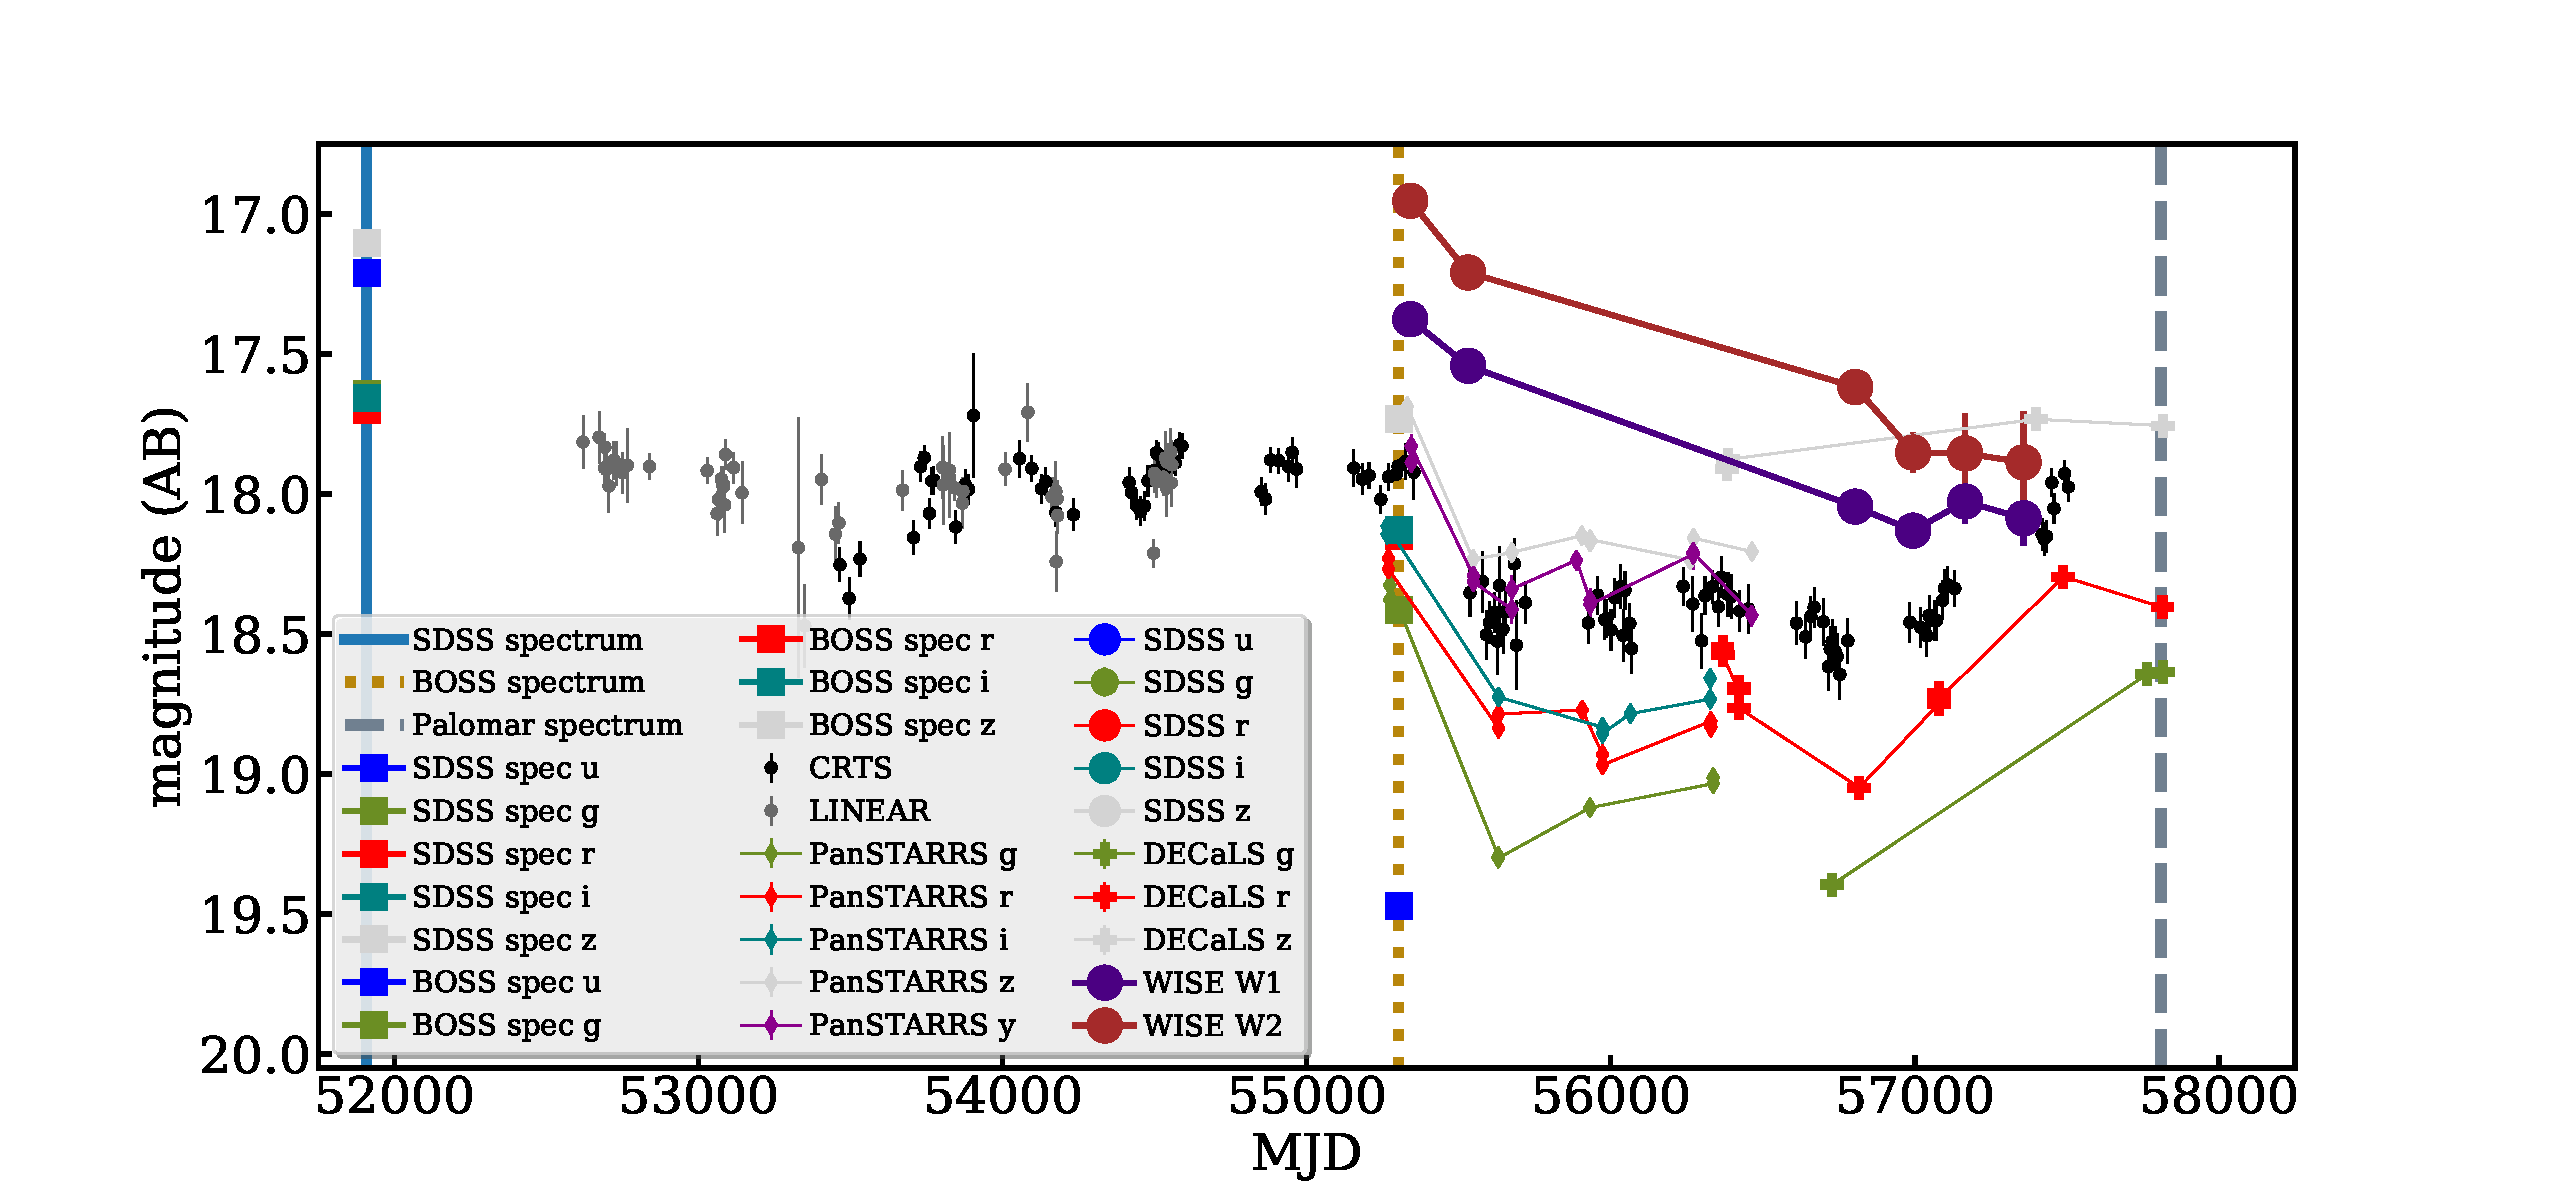
\includegraphics[width=16.00cm, height=7.00cm, trim=0.0cm 0.0cm 0.0cm 0.0cm, clip]
  {../plots/lc/J110057_lc_20171016v2.pdf}
  \caption[]{The light curve of J110057. SDSS, DECaLS and PanSTARRS
    give the optical photometery. The WISE IR light curves are shown and
    their dramatic decrease led to the identification of J110057. The
    three spectral epochs are shown by the vertical lines.}
  \label{fig:J110057_LC_CRTS}
\end{figure*}


\begin{figure*}
  %% trim=l b r t 
  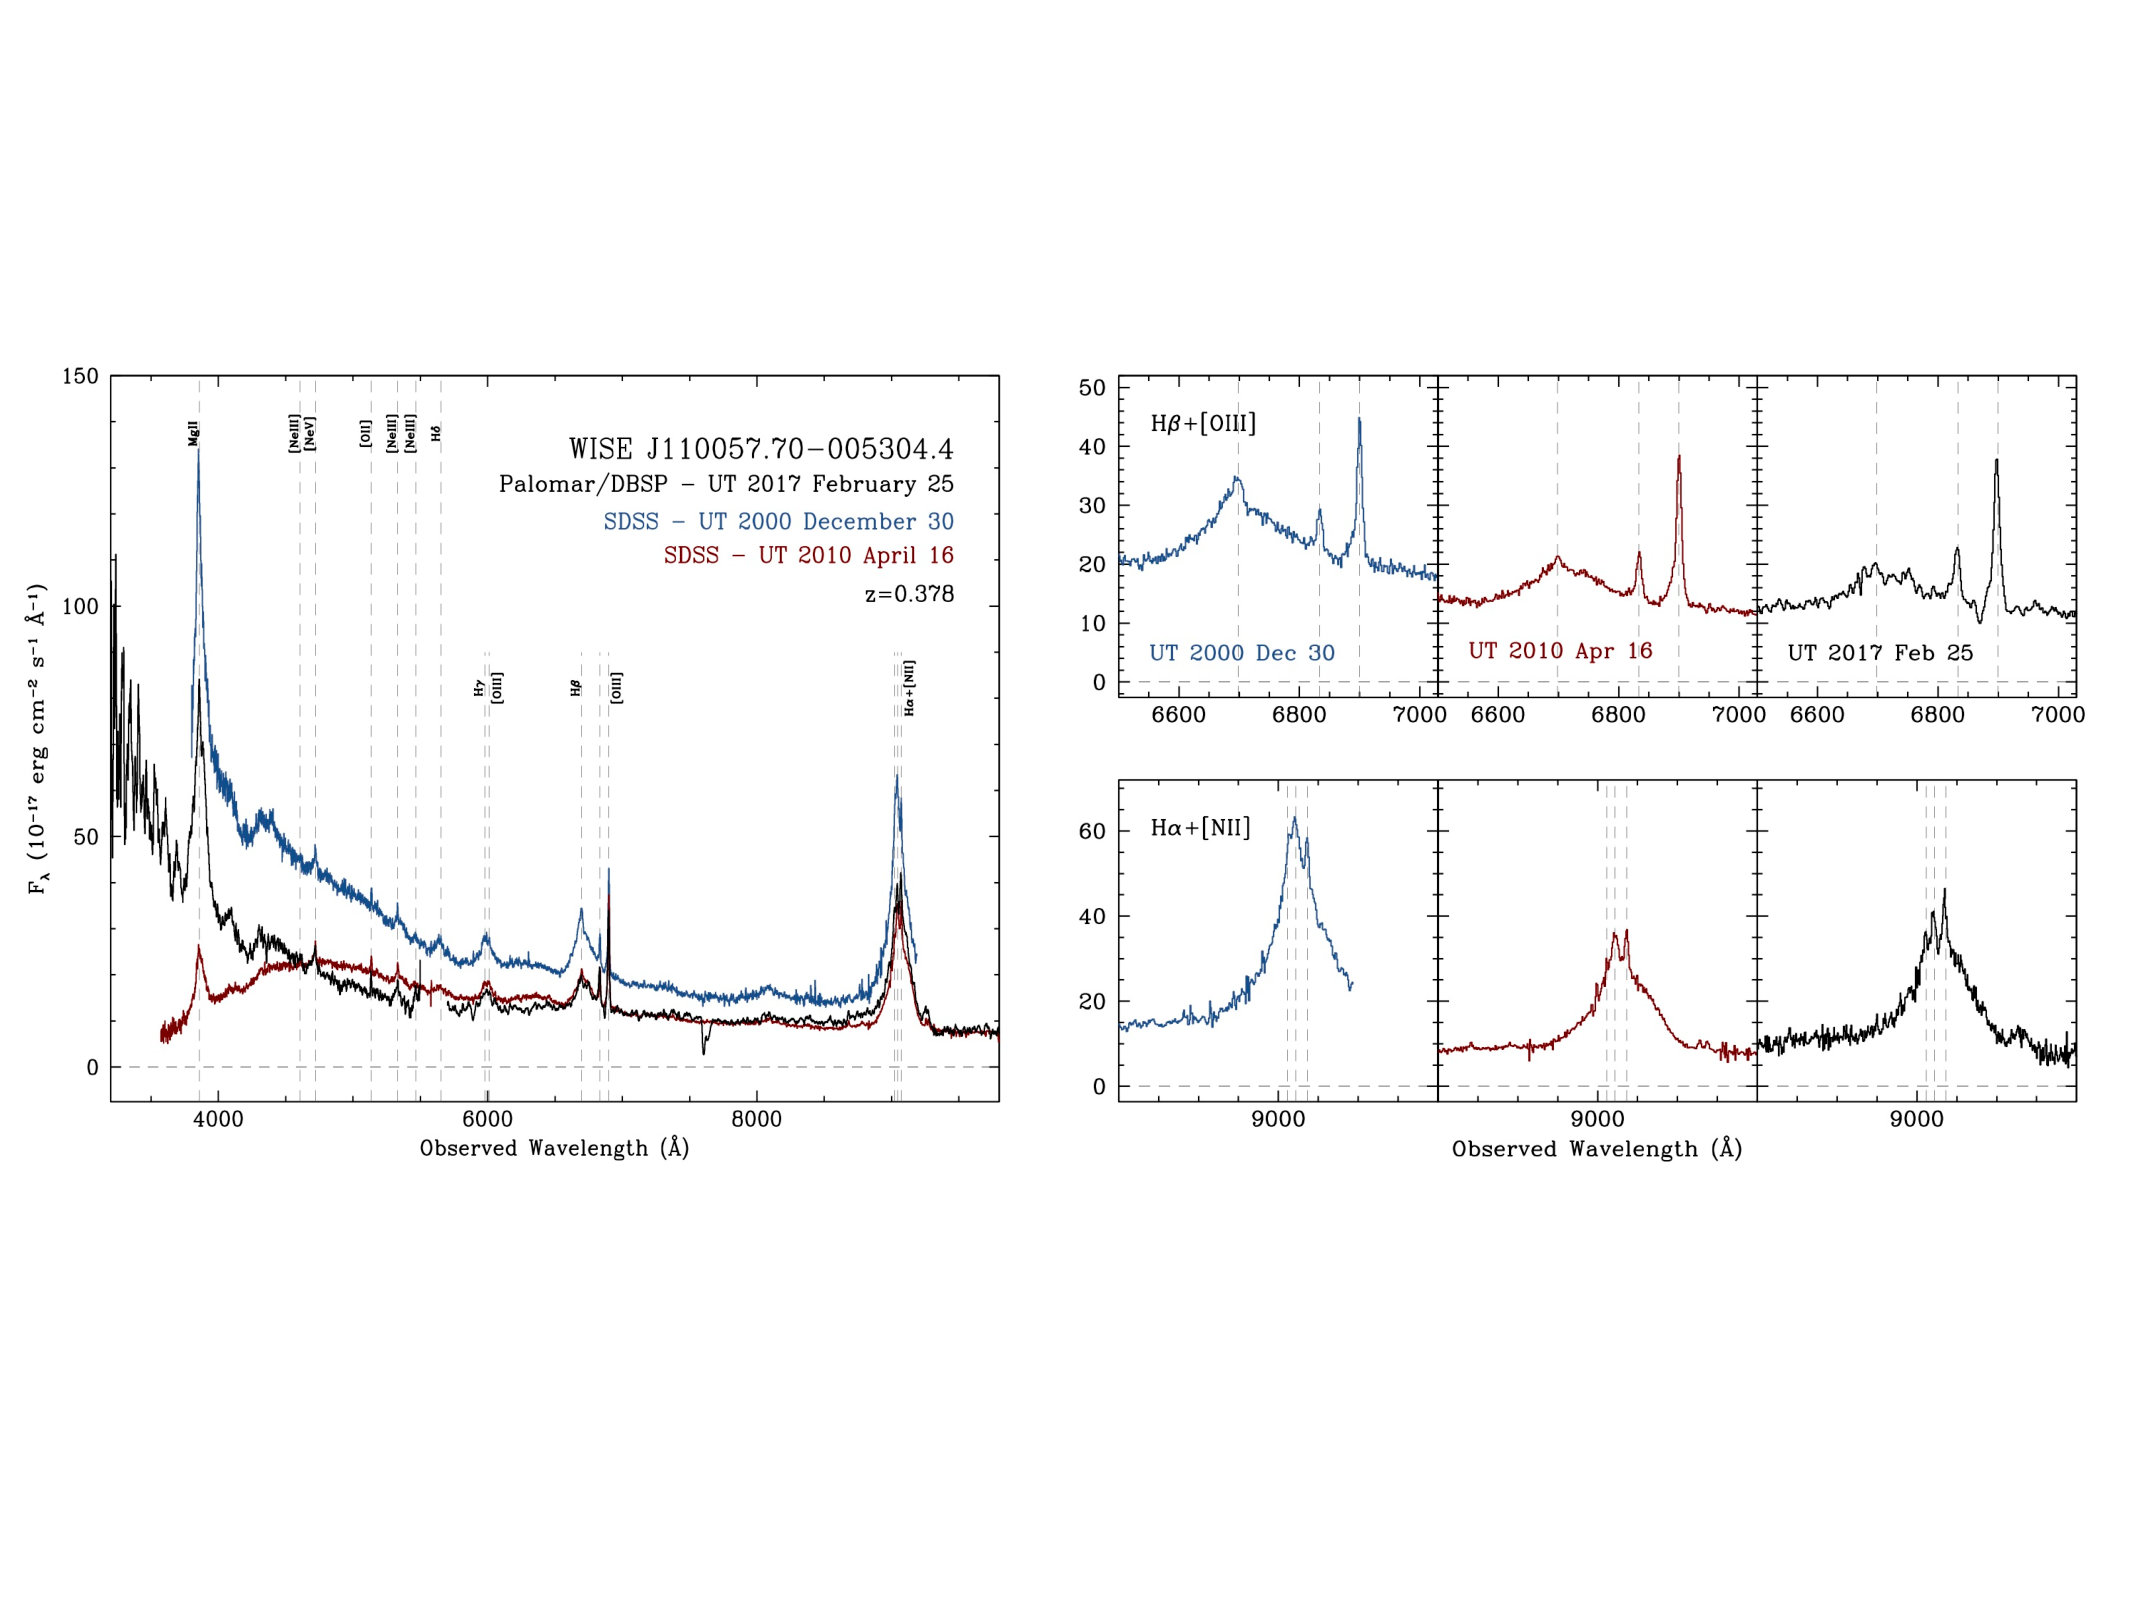
\includegraphics[width=16.00cm, height=7.00cm, trim=0.0cm 0.0cm 0.0cm 0.0cm, clip]
  {../plots/spectra/J110057_spectra_wBalmers.pdf}
  \centering
  \caption[]{
Optical spectra of J110057 obtained on MJD 51908 (blue; SDSS), 55302,
(red; BOSS) and 57809 (black; Palomar/DBSP).  {\it Left::} The full
optical spectra; {\it Right (top)::} Zoom in on the H$\beta$-\oiii
complex; {\it Right (bottom)::} Zoom in on the H$\alpha$-\nii complex.
}
  \label{fig:J110057_spectra}
\end{figure*}
%%%%%%%%%%%%%%%%%%%%%%%%%%%%%%%%%%%%%%%%%%%%%%%%%%%%%%%%%%%%%
%%%%%%%%%%%%%%%%%%%%%%%%%%%%%%%%%%%%%%%%%%%%%%%%%%%%%%%%%%%%%
%%
%%   SECTION 2   SECTION 2   SECTION 2   SECTION 2   SECTION 2   SECTION 2  
%%   SECTION 2   SECTION 2   SECTION 2   SECTION 2   SECTION 2   SECTION 2  
%%   SECTION 2   SECTION 2   SECTION 2   SECTION 2   SECTION 2   SECTION 2  
%%
%%%%%%%%%%%%%%%%%%%%%%%%%%%%%%%%%%%%%%%%%%%%%%%%%%%%%%%%%%%%%
%%%%%%%%%%%%%%%%%%%%%%%%%%%%%%%%%%%%%%%%%%%%%%%%%%%%%%%%%%%%%
\section{Results}  
We started by matching the SDSS-III BOSS Data Release 12 Quasar
catalog \cite[DR12Q; ][]{Paris17)} to the NEOWISE-R IR data (WISE W1
at 3.4$\mu$m, WISE W2 at 4.6$\mu$m) we found $\approx$200 objects with
fading light IR light curves; these objects were identified by a
factor of 2 or more drop in the observed WISE W1 and W2 bands.
Scanning these 200 objects we also examined the change in optical
colour using the SDSS and DECaLS imaging surveys. From this sample of
$\approx$200 QSOs with interesting IR light curves, we obtained new
optical spectroscopy from the Palomar 5m telescope.  J110057 was one
of these 70 objects, but critically, had spectra from both SDSS and
BOSS and hence was a top priority target.

Figure~\ref{fig:J110057_LC_CRTS} gives the optical light curve of
J110057.  Figure~\ref{fig:J110057_spectra} shows the three optical
spectra of J110057. Figure~\ref{fig:J110057_spectra} shows the optical
spectra for J110057 from the SDSS, the BOSS and Palomar observations
taken on MJD 51908, 55302, and 57809. The MJD 51908 SDSS spectrum is
of a typical blue quasar, the blue continuum then collapses.

Checking the data archives we found there was no source within 30
arcsec in the VLA FIRST, i.e., at 21 cm radio frequencies.  None of
the {\it Hubble Space Telescope}, the {\it Spitzer Space Telescope} or
the {\it Kepler} Mission has observed J110057.  It is also not in the
HSC DR1 footprint.  There is a detection in ROSAT, using the 2nd
all-sky survey (2RXS; Boller et al. 2016, A\&A, 588, 103) as 2RXS
J110058.1-005259 with 27.00 counts (count error 6.14) and a count rate
= 0.06$\pm$0.01. The NED gives J110057 as $1.27\pm0.28 \times^{-12}$
erg/cm$^{2}$/s in the 0.1-2.4 keV range (unabsorbed flux). J110057 is
not in either {\it Chandra} or {\it XMM-Newton}.




%%%%%%%%%%%%%%%%%%%%%%%%%%%%%%%%%%%%%%%%%%%%%%%%%%%%%%%%%%%%%
%%%%%%%%%%%%%%%%%%%%%%%%%%%%%%%%%%%%%%%%%%%%%%%%%%%%%%%%%%%%%
%%
%%   SECTION 3   SECTION 3   SECTION 3   SECTION 3   SECTION 3   SECTION 3  
%%   SECTION 3   SECTION 3   SECTION 3   SECTION 3   SECTION 3   SECTION 3  
%%   SECTION 3   SECTION 3   SECTION 3   SECTION 3   SECTION 3   SECTION 3  
%%
%%%%%%%%%%%%%%%%%%%%%%%%%%%%%%%%%%%%%%%%%%%%%%%%%%%%%%%%%%%%%
%%%%%%%%%%%%%%%%%%%%%%%%%%%%%%%%%%%%%%%%%%%%%%%%%%%%%%%%%%%%%
\begin{figure*}
  %% trim=l b r t 
  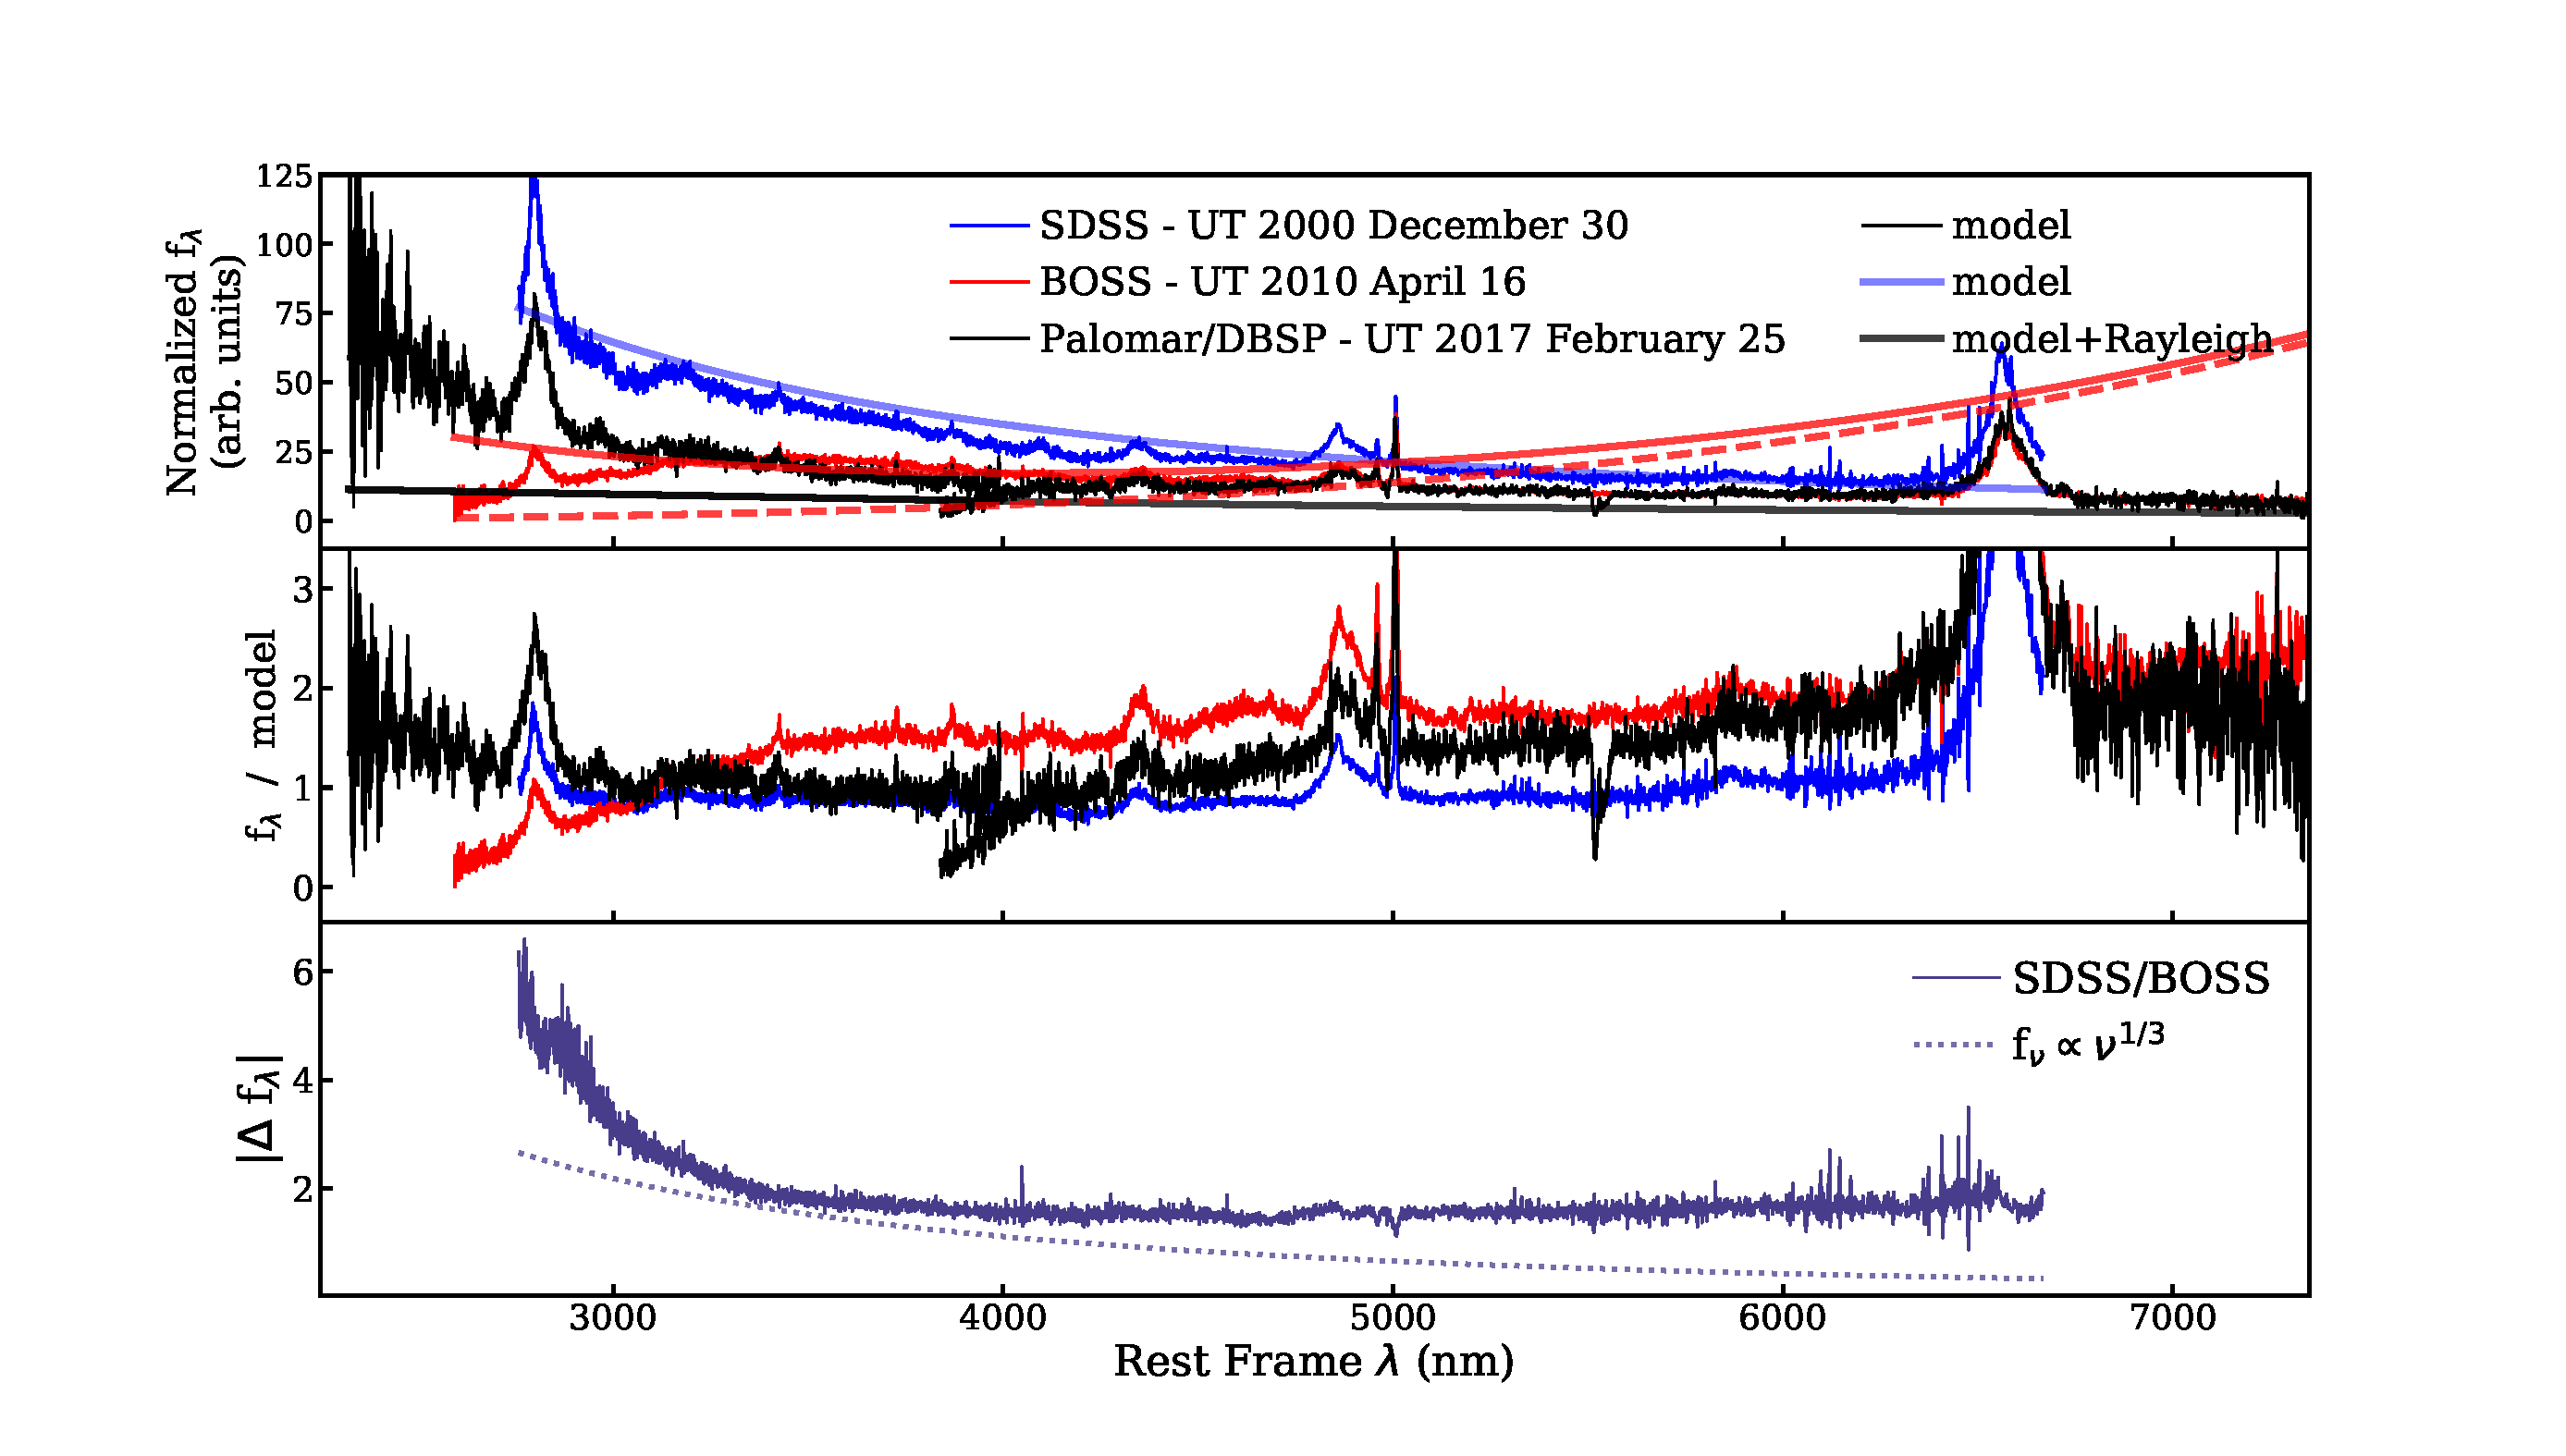
\includegraphics[width=15.4cm, height=8.75cm, trim=0.0cm 0.0cm 0.0cm 0.0cm, clip]
  {../plots/models/mcd_gap_v3_20171017v1.pdf}
  \centering
  \caption[]{The three observed spectra of J110057, with our model
    being overplotted at each spectral epoch. For clarity, the bottom
    panel shows the spectra with the model divided through. }
  \label{fig:J110057_diskmodel}
\end{figure*}
\section{Discussion}   
Using \cite{Sirko_Goodman2003} as our starting point, our preliminary
model (Ford et al.) of emission from a multicolor disk implies changes
in the region from the ISCO to $\sim$few tens-100 $R_{\rm g}$ are
required to suppress flux into the observed $g$-band. In particular,
we suggest a physical collapse of the disk scale height due to a
cooling front propagating outward from the ISCO.

For J110057 we apply our model as follows. We start with an inflated
disk, with non-zero torque at the ISCO, and $h/R\sim0.2$ inside of
$R\sim100 R_{\rm g}$.  This is the initial state in circa 2000
($\approx$ MJD 51900).  Around 2007, there is a switch to a zero
torque at ISCO state. A cooling front is set-up, which propagates out
from the ISCO at the timescale, $t_{\rm front}$. Regions behind the
front emit flux at $\sim$0.1$L$ of what they did prior to the passage
of the front ({\bf NPR comment;: due to drop in T?  T $\downarrow
\times 1.78 \Rightarrow L \downarrow \times10$}), and the temperature
decrease leads the height to drop by a factor of 2.  ({\bf NPR
comment: just due to less kinetic energy??}).  $L_{\rm ion}$ starts
decreasing due to the drop in ionizing photons, which in turn causes
the Balmer lines to also decrease in flux.

If the inner accretion disk is usually inflated \cite[e.g.,
see][]{Sirko_Goodman2003, Thompson2005, Hopkins_Quataert2011}, such a
cooling front will naturally produce: 1) a collapse in the scale
height of the disk; 2) a decrease in flux moving from UV to longer
optical wavelengths; 3) a temporarily thicker scattering atmosphere,
further decreasing flux at short wavelengths.  This model implies
changes to the optical emission moving from shorter to longer
wavelengths (as the radius of the cooling front increases), on
months-to-years-long timescales. It also predicts a longer time to
recover the original flux (compared to the initial collapse, as a
front will move more slowly in a thinner disk (see Fig.~2). A decrease
in the UV flux would also be expected to cause a decrease in IR flux,
as the heating of the IR-emitting dusty torus is reduced; however,
there should also be a delay due to light travel time.

Since the disk starts puffed-up, the cooling front time is not long,
and by 2010 (MJD 55300), the front has reached $R\sim50 R_{g}$. During
that time, the collapsing disk height increases the number density of
scatterers, which in turn causes Rayleigh scattering producing the
blue downturn in the 2010 spectrum.  The cooling front keeps going,
until it hits the part of the disk where it is normally thin, around
$R=100 R_g$, arriving around 2012. This sets up another (heating)
front, which will travel {\it back in} towards the SMBH, and
re-inflate the disk. This `returning' front travels more slowly
because the disk is thinner. It also means the return to normal will
be asymmetric in time, as observed, and the $g$-band bottoms out first
because that is coming from $R\sim100R_{g}$.

Using \citet{Ford2018} and \citet{Sirko_Goodman2003},
Figure~\ref{fig:J110057_diskmodel} shows a model for a $M_{\rm
BH}=3\times 10^{8} M_{\odot}$, radiative efficiency of $\epsilon=0.1$,
accretion rate in units of Eddington accretion, $\dot{M}=0.032$, inner
and outer disk radii in units of $r_g$ of SMBH of radius$_{\rm
in}$=6.0, radius$_{\rm out}$=1.0$\times 10^{4}$. The resulting model
spectra can be seen in Figure~\ref{fig:J110057_diskmodel}.  We expect
the front to return to the ISCO in about 2018. That means the H lines
will come back a few months later, but the WISE IR flux shouldn't come
back until about 2021.

\cite{Guo2016} observed a similar event to J110057, with SDSS J231742.60
+000535.1. However, their object provided an ambiguous case, as the IR
brightness of their source did not decline. However this is consistent
with our model, as their cooling event is relatively brief.




%%%%%%%%%%%%%%%%%%%%%%%%%%%%%%%%%%%%%%%%%%%%%%%%%%%%%%%%%%%%%
%%%%%%%%%%%%%%%%%%%%%%%%%%%%%%%%%%%%%%%%%%%%%%%%%%%%%%%%%%%%%
%%
%%   SECTION 4   SECTION 4   SECTION 4   SECTION 4   SECTION 4   SECTION 4  
%%   SECTION 4   SECTION 4   SECTION 4   SECTION 4   SECTION 4   SECTION 4  
%%   SECTION 4   SECTION 4   SECTION 4   SECTION 4   SECTION 4   SECTION 4  
%%
%%%%%%%%%%%%%%%%%%%%%%%%%%%%%%%%%%%%%%%%%%%%%%%%%%%%%%%%%%%%%
%%%%%%%%%%%%%%%%%%%%%%%%%%%%%%%%%%%%%%%%%%%%%%%%%%%%%%%%%%%%%
%\section{Method}

%\bibliographystyle{naturemag}
%bibliography{/cos_pc19a_npr/LaTeX/tester_mnras}
%\bibliography{sample}



\begin{thebibliography}{10}
\expandafter\ifx\csname url\endcsname\relax
  \def\url#1{\texttt{#1}}\fi
\expandafter\ifx\csname urlprefix\endcsname\relax\def\urlprefix{URL }\fi
\providecommand{\bibinfo}[2]{#2}
\providecommand{\eprint}[2][]{\url{#2}}

\bibitem{LaMassa2015}
\bibinfo{author}{{LaMassa}, S.~M.} \emph{et~al.}
\newblock \bibinfo{title}{{The Discovery of the First ``Changing Look'' Quasar:
  New Insights Into the Physics and Phenomenology of Active Galactic Nucleus}}.
\newblock \emph{\bibinfo{journal}{\apj}} \textbf{\bibinfo{volume}{800}},
  \bibinfo{pages}{144} (\bibinfo{year}{2015}).
\newblock \eprint{1412.2136}.

\bibitem{Runnoe2016}
\bibinfo{author}{{Runnoe}, J.~C.} \emph{et~al.}
\newblock \bibinfo{title}{{Now you see it, now you don't: the disappearing
  central engine of the quasar J1011+5442}}.
\newblock \emph{\bibinfo{journal}{\mnras}} \textbf{\bibinfo{volume}{455}},
  \bibinfo{pages}{1691--1701} (\bibinfo{year}{2016}).
\newblock \eprint{1509.03640}.

\bibitem{MacLeod2016}
\bibinfo{author}{{MacLeod}, C.~L.} \emph{et~al.}
\newblock \bibinfo{title}{{A systematic search for changing-look quasars in
  SDSS}}.
\newblock \emph{\bibinfo{journal}{\mnras}} \textbf{\bibinfo{volume}{457}},
  \bibinfo{pages}{389--404} (\bibinfo{year}{2016}).
\newblock \eprint{1509.08393}.

\bibitem{Ruan2016}
\bibinfo{author}{{Ruan}, J.~J.} \emph{et~al.}
\newblock \bibinfo{title}{{Toward an Understanding of Changing-look Quasars: An
  Archival Spectroscopic Search in SDSS}}.
\newblock \emph{\bibinfo{journal}{\apj}} \textbf{\bibinfo{volume}{826}},
  \bibinfo{pages}{188} (\bibinfo{year}{2016}).
\newblock \eprint{1509.03634}.

\bibitem{Hutsemekers2017}
\bibinfo{author}{{Hutsem{\'e}kers}, D.}, \bibinfo{author}{{Ag{\'{\i}}s
  Gonz{\'a}lez}, B.}, \bibinfo{author}{{Sluse}, D.}, \bibinfo{author}{{Ramos
  Almeida}, C.} \& \bibinfo{author}{{Acosta Pulido}, J.-A.}
\newblock \bibinfo{title}{{Polarization of the changing-look quasar
  J1011+5442}}.
\newblock \emph{\bibinfo{journal}{\aap}} \textbf{\bibinfo{volume}{604}},
  \bibinfo{pages}{L3} (\bibinfo{year}{2017}).
\newblock \eprint{1707.05540}.

\bibitem{Sheng2017}
\bibinfo{author}{{Sheng}, Z.} \emph{et~al.}
\newblock \bibinfo{title}{{Mid-infrared Variability of Changing-look AGNs}}.
\newblock \emph{\bibinfo{journal}{\apjl}} \textbf{\bibinfo{volume}{846}},
  \bibinfo{pages}{L7} (\bibinfo{year}{2017}).
\newblock \eprint{1707.02686}.

\bibitem{Gezari2017}
\bibinfo{author}{{Gezari}, S.} \emph{et~al.}
\newblock \bibinfo{title}{{iPTF Discovery of the Rapid ``Turn-on'' of a
  Luminous Quasar}}.
\newblock \emph{\bibinfo{journal}{\apj}} \textbf{\bibinfo{volume}{835}},
  \bibinfo{pages}{144} (\bibinfo{year}{2017}).
\newblock \eprint{1612.04830}.

\bibitem{Rumbaugh2017}
\bibinfo{author}{{Rumbaugh}, N.} \emph{et~al.}
\newblock \bibinfo{title}{{Extreme variability quasars from the Sloan Digital
  Sky Survey and the Dark Energy Survey}}.
\newblock \emph{\bibinfo{journal}{ArXiv e-prints}}  (\bibinfo{year}{2017}).
\newblock \eprint{1706.07875}.

\bibitem{SS73}
\bibinfo{author}{{Shakura}, N.~I.} \& \bibinfo{author}{{Sunyaev}, R.~A.}
\newblock \bibinfo{title}{{Black holes in binary systems. Observational
  appearance.}}
\newblock \emph{\bibinfo{journal}{\aap}} \textbf{\bibinfo{volume}{24}},
  \bibinfo{pages}{337} (\bibinfo{year}{1973}).

\bibitem{Antonucci1999}
\bibinfo{author}{{Antonucci}, R.}
\newblock \bibinfo{title}{{Constraints on Disks Models of The Big Blue Bump
  from UV/Optical/IR Observations}}.
\newblock In \bibinfo{editor}{{Poutanen}, J.} \& \bibinfo{editor}{{Svensson},
  R.} (eds.) \emph{\bibinfo{booktitle}{High Energy Processes in Accreting Black
  Holes}}, vol. \bibinfo{volume}{161} of \emph{\bibinfo{series}{Astronomical
  Society of the Pacific Conference Series}}, \bibinfo{pages}{193}
  (\bibinfo{year}{1999}).
\newblock \eprint{astro-ph/9810067}.

\bibitem{Koratkar_Blaes1999}
\bibinfo{author}{{Koratkar}, A.} \& \bibinfo{author}{{Blaes}, O.}
\newblock \bibinfo{title}{{The Ultraviolet and Optical Continuum Emission in
  Active Galactic Nuclei: The Status of Accretion Disks}}.
\newblock \emph{\bibinfo{journal}{\pasp}} \textbf{\bibinfo{volume}{111}},
  \bibinfo{pages}{1--30} (\bibinfo{year}{1999}).

\bibitem{Lawrence2012}
\bibinfo{author}{{Lawrence}, A.}
\newblock \bibinfo{title}{{The UV peak in active galactic nuclei: a false
  continuum from blurred reflection?}}
\newblock \emph{\bibinfo{journal}{\mnras}} \textbf{\bibinfo{volume}{423}},
  \bibinfo{pages}{451--463} (\bibinfo{year}{2012}).
\newblock \eprint{1110.0854}.

\bibitem{Pooley2007}
\bibinfo{author}{{Pooley}, D.}, \bibinfo{author}{{Blackburne}, J.~A.},
  \bibinfo{author}{{Rappaport}, S.} \& \bibinfo{author}{{Schechter}, P.~L.}
\newblock \bibinfo{title}{{X-Ray and Optical Flux Ratio Anomalies in Quadruply
  Lensed Quasars. I. Zooming in on Quasar Emission Regions}}.
\newblock \emph{\bibinfo{journal}{\apj}} \textbf{\bibinfo{volume}{661}},
  \bibinfo{pages}{19--29} (\bibinfo{year}{2007}).
\newblock \eprint{astro-ph/0607655}.

\bibitem{Morgan2010}
\bibinfo{author}{{Morgan}, C.~W.}, \bibinfo{author}{{Kochanek}, C.~S.},
  \bibinfo{author}{{Morgan}, N.~D.} \& \bibinfo{author}{{Falco}, E.~E.}
\newblock \bibinfo{title}{{The Quasar Accretion Disk Size-Black Hole Mass
  Relation}}.
\newblock \emph{\bibinfo{journal}{\apj}} \textbf{\bibinfo{volume}{712}},
  \bibinfo{pages}{1129--1136} (\bibinfo{year}{2010}).
\newblock \eprint{1002.4160}.

\bibitem{Morgan2012}
\bibinfo{author}{{Morgan}, C.~W.} \emph{et~al.}
\newblock \bibinfo{title}{{Further Evidence that Quasar X-Ray Emitting Regions
  are Compact: X-Ray and Optical Microlensing in the Lensed Quasar Q
  J0158-4325}}.
\newblock \emph{\bibinfo{journal}{\apj}} \textbf{\bibinfo{volume}{756}},
  \bibinfo{pages}{52} (\bibinfo{year}{2012}).
\newblock \eprint{1205.4727}.

\bibitem{Mosquera2011}
\bibinfo{author}{{Mosquera}, A.~M.} \& \bibinfo{author}{{Kochanek}, C.~S.}
\newblock \bibinfo{title}{{The Microlensing Properties of a Sample of 87 Lensed
  Quasars}}.
\newblock \emph{\bibinfo{journal}{\apj}} \textbf{\bibinfo{volume}{738}},
  \bibinfo{pages}{96} (\bibinfo{year}{2011}).
\newblock \eprint{1104.2356}.

\bibitem{Mainzer2014}
\bibinfo{author}{{Mainzer}, A.} \emph{et~al.}
\newblock \bibinfo{title}{{Initial Performance of the NEOWISE Reactivation
  Mission}}.
\newblock \emph{\bibinfo{journal}{\apj}} \textbf{\bibinfo{volume}{792}},
  \bibinfo{pages}{30} (\bibinfo{year}{2014}).
\newblock \eprint{1406.6025}.

\bibitem{Meisner2017}
\bibinfo{author}{{Meisner}, A.~M.}, \bibinfo{author}{{Lang}, D.} \&
  \bibinfo{author}{{Schlegel}, D.~J.}
\newblock \bibinfo{title}{{Deep Full-sky Coadds from Three Years of WISE and
  NEOWISE Observations}}.
\newblock \emph{\bibinfo{journal}{\aj}} \textbf{\bibinfo{volume}{154}},
  \bibinfo{pages}{161} (\bibinfo{year}{2017}).
\newblock \eprint{1705.06746}.

\bibitem{Meisner2017b}
\bibinfo{author}{{Meisner}, A.~M.} \emph{et~al.}
\newblock \bibinfo{title}{{Searching for Planet Nine with Coadded WISE and
  NEOWISE-Reactivation Images}}.
\newblock \emph{\bibinfo{journal}{\aj}} \textbf{\bibinfo{volume}{153}},
  \bibinfo{pages}{65} (\bibinfo{year}{2017}).
\newblock \eprint{1611.00015}.

\bibitem{Guo2016}
\bibinfo{author}{{}, H.} \emph{et~al.}
\newblock \bibinfo{title}{{The Optical Variability of SDSS Quasars from
  Multi-epoch Spectroscopy. III. A Sudden UV Cutoff in Quasar SDSS
  J2317+0005}}.
\newblock \emph{\bibinfo{journal}{\apj}} \textbf{\bibinfo{volume}{826}},
  \bibinfo{pages}{186} (\bibinfo{year}{2016}).
\newblock \eprint{1605.07301}.

\end{thebibliography}



\end{document}
